\documentclass{article}
\usepackage[preprint,nonatbib]{neurips_2025}

\usepackage[utf8]{inputenc}
\usepackage[T5]{fontenc}
\usepackage[vietnamese]{babel}
\usepackage{hyperref}
\usepackage{url}
\usepackage{booktabs}
\usepackage{amsmath}
\usepackage{graphicx}
\usepackage{subcaption}
\usepackage{xcolor}
\usepackage{microtype}

\title{Dự Báo Doanh Thu và Giá Vốn Theo Ngày bằng Ensemble Gradient Boosting Theo Thời Gian}

\author{%
  Impact\\
  VinUni Datathon 2026\\
  \texttt{forecasting report}
}

\begin{document}
\maketitle

\begin{abstract}
Báo cáo này trình bày pipeline dự báo doanh thu (Revenue) và giá vốn hàng bán (COGS) theo ngày. Hệ thống sử dụng bảng sales tổng hợp theo ngày, nhóm đặc trưng lịch có thể biết trước trong tương lai, cross-validation đúng chiều thời gian, và ensemble gồm LightGBM, XGBoost, CatBoost được huấn luyện trên target đã biến đổi log. Ở bước suy luận, dự báo được lấy trung bình qua nhiều model và nhiều fold, sau đó áp dụng các ràng buộc nghiệp vụ để đảm bảo dự báo không âm và \(\mathrm{COGS} \leq \mathrm{Revenue}\). Phần giải thích mô hình được thực hiện bằng SHAP trên thành phần LightGBM đại diện cho nhóm mô hình cây trong ensemble.
\end{abstract}

\section{Giới thiệu}
Bài toán yêu cầu dự báo Revenue và COGS theo ngày cho giai đoạn tương lai từ 2023-01-01 đến 2024-07-01 dựa trên dữ liệu lịch sử. Một pipeline phù hợp cho bài toán này cần thỏa mãn bốn yêu cầu chính: giữ đúng thứ tự thời gian khi validation, tránh rò rỉ thông tin từ tương lai, tạo đầu ra hợp lệ về mặt nghiệp vụ, và có khả năng giải thích các yếu tố chính ảnh hưởng đến dự báo.

Hướng tiếp cận cuối cùng được thiết kế theo nguyên tắc đơn giản và ổn định. Thay vì dùng dự báo đệ quy dựa trên lag/rolling, vốn có thể tích lũy sai số trong horizon dài, pipeline dự báo trực tiếp từ các đặc trưng lịch tĩnh. Những đặc trưng này tồn tại cả ở train và test, nhờ đó giảm rủi ro phải giả lập các biến tương lai không chắc chắn.

\section{Trực quan hóa và phân tích dữ liệu}
Bảng forecasting chính gồm 3,833 quan sát theo ngày từ 2012-07-04 đến 2022-12-31 với ba cột: Date, Revenue và COGS. File submission mẫu gồm 548 ngày tương lai từ 2023-01-01 đến 2024-07-01. Các cột bắt buộc trong bảng train không có giá trị thiếu. Doanh thu trung bình trong lịch sử là khoảng 4.29 triệu, COGS trung bình khoảng 3.70 triệu, và tỷ lệ COGS/Revenue trung bình là 0.875.

Hình~\ref{fig:eda} tóm tắt các quan sát quan trọng từ EDA. Revenue và COGS có cấu trúc biến động khá tương đồng, vì vậy hai target có thể dùng cùng một bộ đặc trưng và protocol huấn luyện. Tổng hợp theo tháng cho thấy yếu tố mùa vụ lặp lại; tổng hợp theo ngày trong tuần cho thấy weekday/weekend là tín hiệu cần giữ lại. Phân phối COGS/Revenue tập trung quanh một vùng chính nhưng vẫn có một số ngày lịch sử mà COGS vượt Revenue, do đó bước post-processing cần ép ràng buộc \(\mathrm{COGS} \leq \mathrm{Revenue}\) cho đầu ra cuối cùng.

\begin{figure}[t]
  \centering
  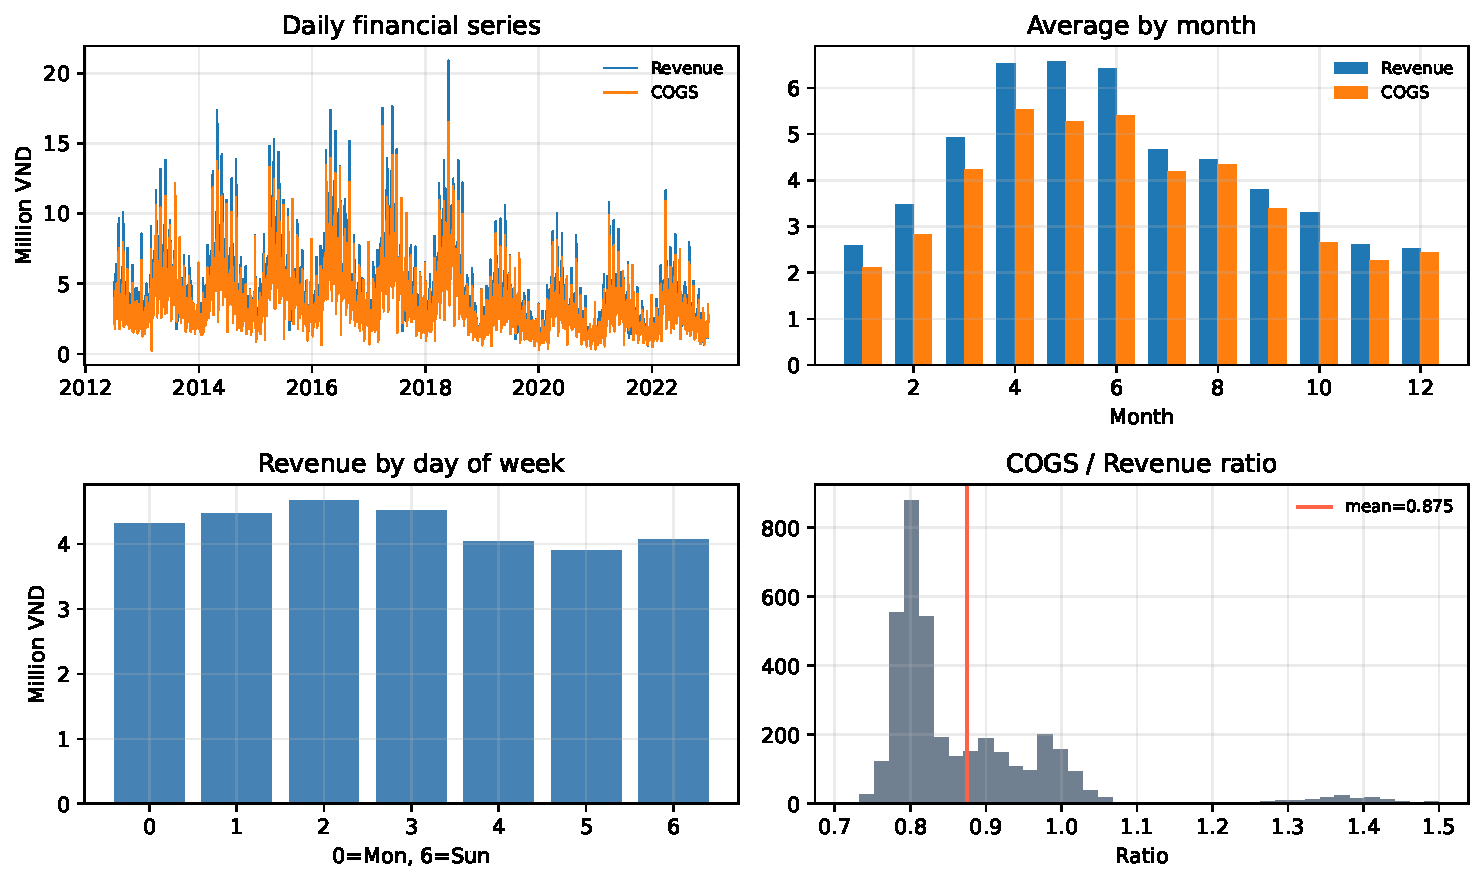
\includegraphics[width=0.96\linewidth]{figures/eda_overview.pdf}
  \caption{Tổng quan EDA trên bảng sales theo ngày: chuỗi Revenue/COGS, mùa vụ theo tháng, hiệu ứng ngày trong tuần, và phân phối tỷ lệ COGS/Revenue.}
  \label{fig:eda}
\end{figure}

\section{Phương pháp tiếp cận và pipeline mô hình}
\paragraph{Feature engineering.}
Với mỗi ngày \(t\), vector đặc trưng gồm mười biến xác định từ lịch: year, month, day, day of week, weekend flag, day of year, quarter, payday flag, và hai biến cyclic month encoding \(\sin(2\pi m/12)\), \(\cos(2\pi m/12)\). Đây là các đặc trưng an toàn với leakage vì chúng được biết trước cho cả giai đoạn tương lai và không phụ thuộc vào Revenue/COGS của các ngày cần dự báo.

\paragraph{Mô hình.}
Revenue và COGS được huấn luyện riêng. Với mỗi target \(y\), model học trên \(\log(1+y)\) và khi dự báo thì chuyển ngược về scale gốc bằng \(\exp(\hat{y})-1\). Ba mô hình được sử dụng là LightGBM, XGBoost và CatBoost. Cả ba đều là gradient boosting tree models mạnh cho dữ liệu dạng bảng, nhưng khác nhau ở cách xây cây và regularization, nên simple averaging giúp giảm phụ thuộc vào một thuật toán đơn lẻ.

\paragraph{Cross-validation theo thời gian.}
Pipeline dùng \texttt{TimeSeriesSplit} với 5 fold. Ở mỗi fold, tập train luôn nằm trước tập validation theo trục thời gian, còn validation là một block ngày nằm sau. Cách chia này phù hợp với bài toán forecasting hơn random K-fold, vì random split có thể để thông tin từ tương lai xuất hiện trong quá trình đánh giá.

\paragraph{Inference và ràng buộc.}
Trên giai đoạn test, dự báo được lấy trung bình qua toàn bộ model và fold. Sau đó pipeline áp dụng hai ràng buộc nghiệp vụ: Revenue/COGS không âm và COGS không vượt Revenue:
\begin{equation}
\widehat{\mathrm{Revenue}} = \max(0, \widehat{\mathrm{Revenue}}), \quad
\widehat{\mathrm{COGS}} = \min\{\max(0, \widehat{\mathrm{COGS}}), \widehat{\mathrm{Revenue}}\}.
\end{equation}
Nhờ vậy file dự báo cuối cùng luôn hợp lệ về mặt tài chính và không cần chỉnh sửa thủ công sau khi export.

\section{Kết quả thực nghiệm và giải thích mô hình}
Bảng~\ref{tab:cv} trình bày metric trung bình trên 5 fold theo thời gian. WAPE được dùng để đánh giá sai số tương đối theo quy mô target, trong khi MAE và RMSE cho biết độ lớn sai số tuyệt đối. LightGBM là single model tốt nhất trên cả Revenue và COGS trong validation nội bộ, nhưng pipeline cuối vẫn giữ cả ba model vì ensemble trung bình thường ổn định hơn trên horizon dài.

\begin{table}[h]
  \caption{Metric validation trung bình trên 5 fold theo thứ tự thời gian.}
  \label{tab:cv}
  \centering
  \small
  \begin{tabular}{llrrr}
    \toprule
    Target & Model & WAPE (\%) & MAE & RMSE \\
    \midrule
    Revenue & LightGBM & 24.36 & 1,013,506 & 1,395,708 \\
    Revenue & XGBoost & 25.49 & 1,057,277 & 1,457,064 \\
    Revenue & CatBoost & 25.26 & 1,047,588 & 1,454,004 \\
    COGS & LightGBM & 23.03 & 824,641 & 1,135,653 \\
    COGS & XGBoost & 23.76 & 854,926 & 1,171,403 \\
    COGS & CatBoost & 23.92 & 853,686 & 1,196,121 \\
    \bottomrule
  \end{tabular}
\end{table}

File submission cuối cùng có 548 dòng, không có missing value, không có dự báo âm, và không có dòng nào vi phạm \(\mathrm{COGS} \leq \mathrm{Revenue}\). Điều này xác nhận rằng pipeline không chỉ tạo dự báo mà còn tuân thủ đầy đủ các ràng buộc đầu ra cần thiết.

\paragraph{Giải thích bằng SHAP.}
Để giải thích mô hình, báo cáo sử dụng SHAP values trên LightGBM của fold cuối. Đây là thành phần đại diện cho nhóm mô hình cây trong ensemble, không phải một model tách rời khỏi pipeline. Hình~\ref{fig:shap} cho thấy các đặc trưng lịch như vị trí trong năm, tháng, payday và weekday/weekend là những yếu tố quan trọng. Kết quả này phù hợp với EDA: tín hiệu chính của bài toán đến từ mùa vụ và cấu trúc lịch, thay vì các biến không chắc chắn trong tương lai.

\begin{figure}[t]
  \centering
  \begin{subfigure}{0.49\linewidth}
    \centering
    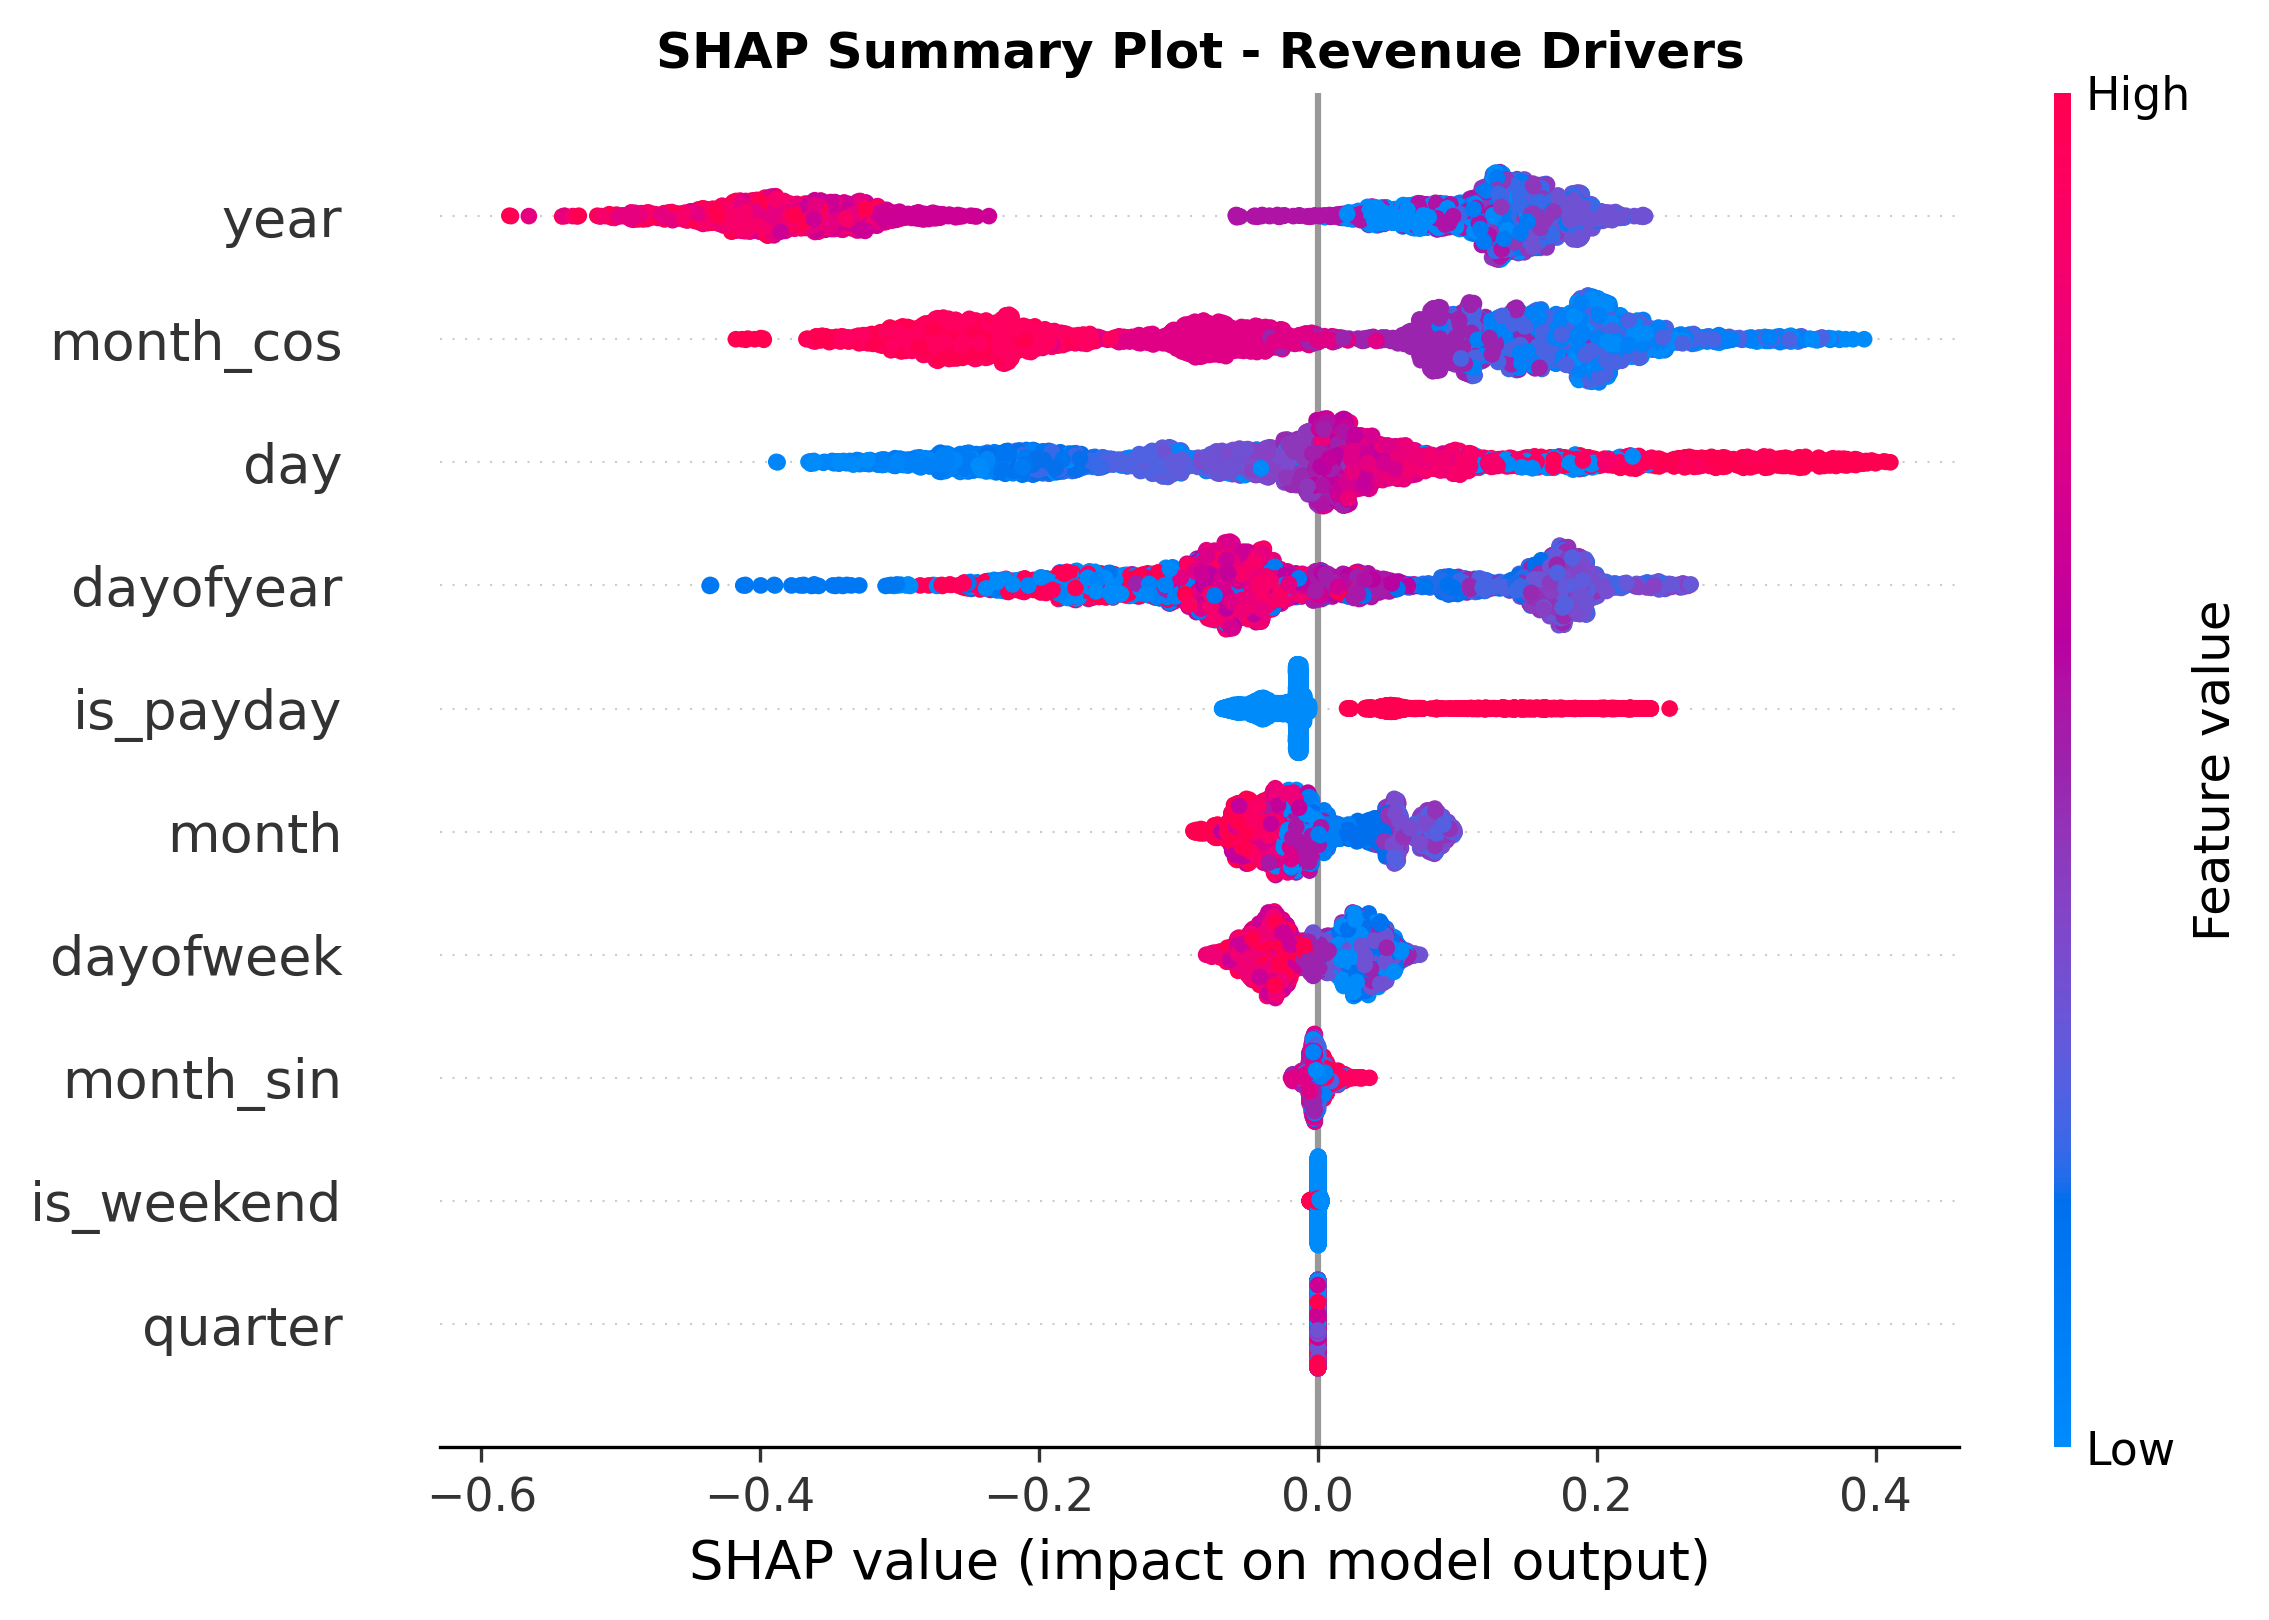
\includegraphics[width=\linewidth]{../models/shap_revenue_drivers.png}
    \caption{Revenue}
  \end{subfigure}
  \hfill
  \begin{subfigure}{0.49\linewidth}
    \centering
    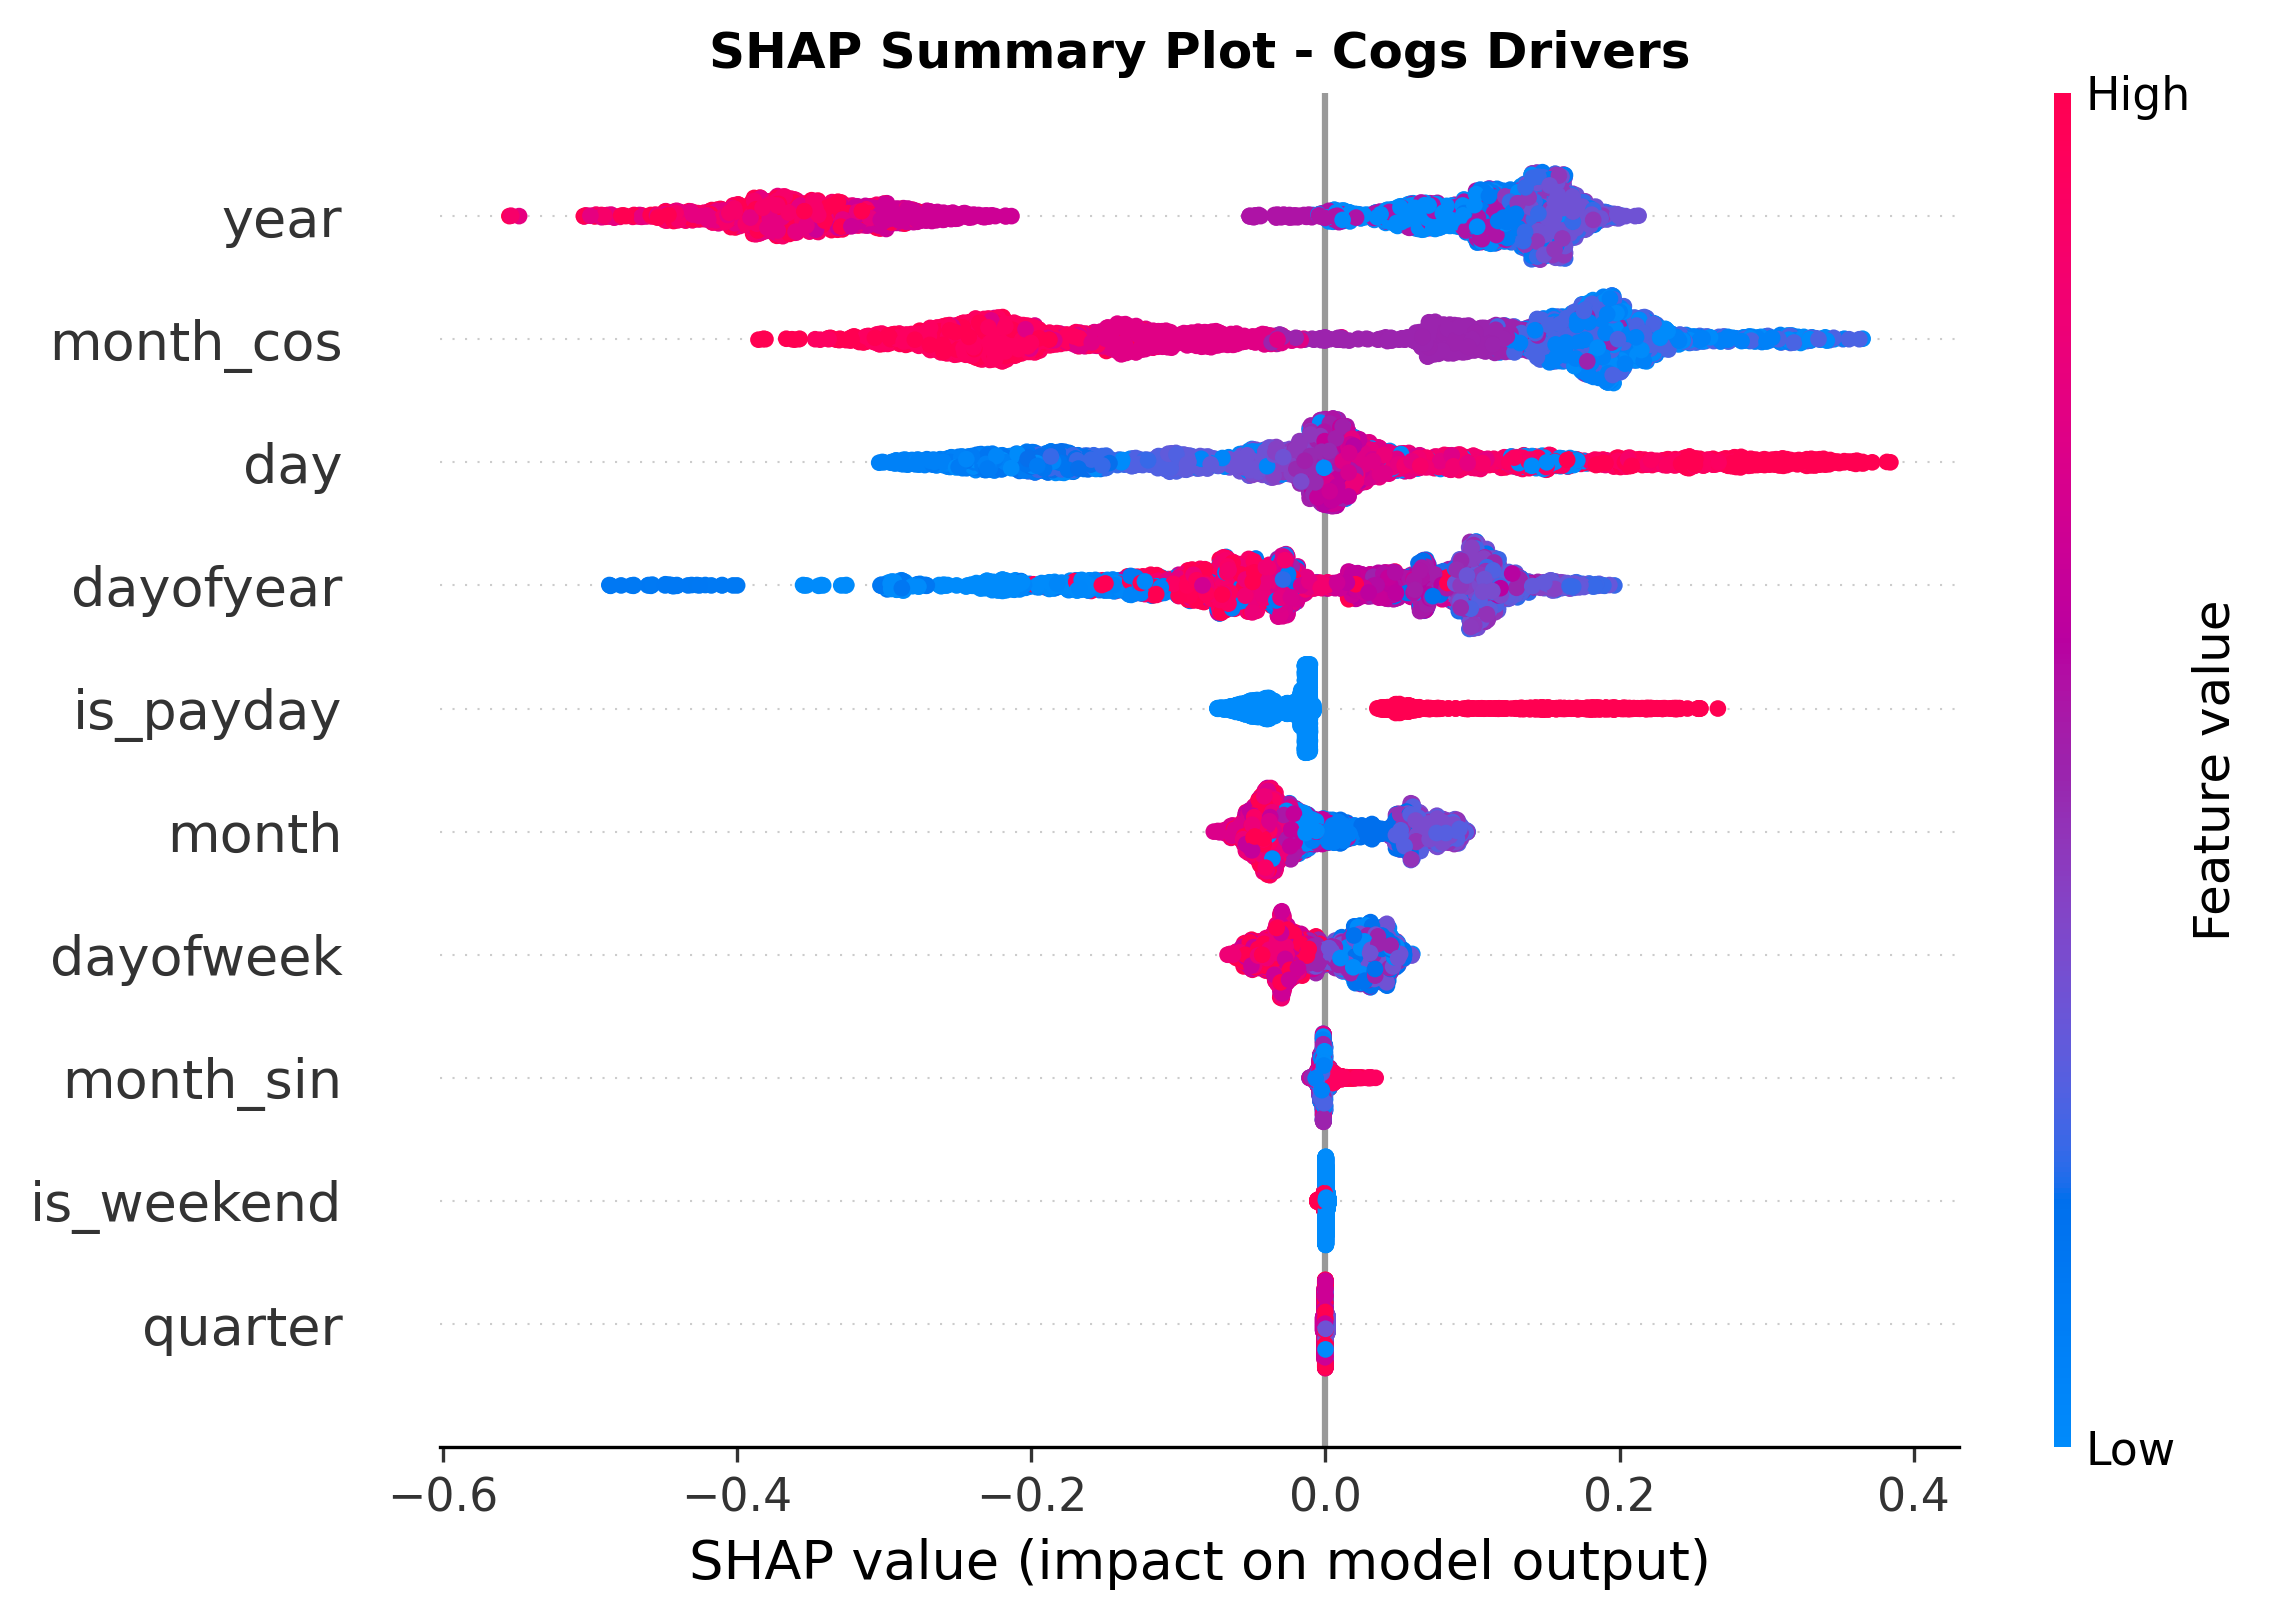
\includegraphics[width=\linewidth]{../models/shap_cogs_drivers.png}
    \caption{COGS}
  \end{subfigure}
  \caption{SHAP summary plots cho LightGBM component trong ensemble.}
  \label{fig:shap}
\end{figure}

\section{Kết luận}
Pipeline cuối ưu tiên tính đúng đắn theo thời gian, feature an toàn với leakage, mô hình tabular mạnh và ràng buộc nghiệp vụ rõ ràng. Direct forecasting trên log-target giúp tránh tích lũy sai số của recursive forecasting, trong khi TimeSeriesSplit tạo quy trình validation sát với bài toán dự báo tương lai. SHAP bổ sung khả năng giải thích, cho thấy model chủ yếu dựa vào các hiệu ứng lịch và mùa vụ. Trong các vòng cải tiến tiếp theo, các nhóm feature phức tạp hơn nên được đưa vào bằng ablation có kiểm soát để tránh distribution shift giữa train và test.

\section*{References}
{\small
[1] Chen, T. and Guestrin, C. (2016). XGBoost: A scalable tree boosting system. \emph{KDD}.\\
[2] Ke, G. et al. (2017). LightGBM: A highly efficient gradient boosting decision tree. \emph{NeurIPS}.\\
[3] Prokhorenkova, L. et al. (2018). CatBoost: unbiased boosting with categorical features. \emph{NeurIPS}.\\
[4] Lundberg, S. and Lee, S.-I. (2017). A unified approach to interpreting model predictions. \emph{NeurIPS}.\\
[5] NeurIPS. (2025). Paper formatting instructions and LaTeX style file. \url{https://neurips.cc/Conferences/2025/CallForPapers}.
}

\appendix
\section{Chi tiết tái lập}
Pipeline có thể chạy từ thư mục gốc project bằng lệnh:
\begin{verbatim}
conda run -n datathon python main.py --data-dir data --output-dir models
\end{verbatim}
Các thư viện cần thiết nằm trong \texttt{requirements.txt}. Các file nguồn chính gồm \texttt{src/data\_loader.py}, \texttt{src/feature\_engineering.py}, \texttt{src/models.py}, và \texttt{src/train.py}.

\end{document}
